\documentclass[shortpaper]{revdetua}

\usepackage{scicite}
\usepackage{hyperref}

\usepackage{amsmath}
\usepackage{multicol}
\usepackage{setspace}

\usepackage{enumitem}

\usepackage{graphicx}
\usepackage{caption}
\usepackage{float}
\usepackage{subcaption}

\usepackage{verbatim}

\usepackage{booktabs}

%%%%%%%%%%%%%%%%%%%%%%%%%%%%%%%%%%%%%%%%%%%%%%%%%%%%%%%%%%%%%%%%%%%%%%%%%%%%%%%%

\begin{document}
 
\Header{2}{85122}{Dezembro}{2019}{1}

\title{
    \LARGE{{\bf Project 3: Frequent Items Counting \/}}
    \vspace{-20pt}
}

\author{
    \Large{{\bf A Study on Memory-Efficient Algorithms\/}}\\\\\\
    Filipe Pires [85122] \& João Alegria [85048]\\
    \\
    {\bf Advanced Algorithms\/}\\
    \normalsize{Department of Electronics, Telecommunications and Informatics}\\
    \normalsize{University of Aveiro}\\
} 

\maketitle

%%%%%%%%%%%%%%%%%%%%%%%%%%%%%%%%%%%%%%%%%%%%%%%%%%%%%%%%%%%%%%%%%%%%%%%%%%%%%%%%

\begin{abstract}
    Lorem ipsum ...
\end{abstract}

\begin{keywords}
    Probabilistic Counter, Count-Min Sketch, Memory-Efficient Algorithms
\end{keywords}

%%%%%%%%%%%%%%%%%%%%%%%%%%%%%%%%%%%%%%%%%%%%%%%%%%%%%%%%%%%%%%%%%%%%%%%%%%%%%%%%

\section{Problem Contextualization}\label{problem}

This report was written for the course of 'Advanced Algorithms', taught by 
professor Joaquim Madeira for the master's in Informatics Engineering at DETI UA.
It describes the work done for the third assignment of the course \cite{trab3}.
The chosen hypothesis was "Hipótese A-2 – Contagem dos Itens Mais Frequentes".

One of the subjects studied in this course was the counting problems and the obstacles that appear when dealing with this type of problems in very large contexts. The difficulties appear even more when the contexts morph into the newest, fastest and the form that delivers the most amount of information, the data streams. Being a continuous source of real time events, processing the events that happen in a precise and reliable way can be more ofter than not very challenging and sometimes impossible. Many solutions appear in hopes of creating reliable approximations that without using the as many resources still permit inferring the same conclusions. This solutions use many times probabilistic approaches or some kind of mapping that allows some form of overlapping of the data without compromising the results, such as hashing. 

This theme was already a subject for previous works, but since it is an area so vast and with so many different approaches, each one with its advantages and disadvantages, the professor decided to list it again for the possible report themes in this last project, but this time with more complex and refined algorithms that use memory and resources in a more intelligent way. We ended up choosing this theme since we are interested in knowing how lower can the resource usage go without compromising the outcome of the model, meaning that the conclusions taken from the approximations made by the model are not too distant from the ones taken from the exact counters.

In the context of literary works as source of text, we create data streams to simulate a real world scenario and test the effectiveness and performance of one of the proposed algorithms. Some of those proposed algorithms were the one from Misra \& Gries(Frequent-Count), the one from Manku \& Motwani(SLossy-Count), the one from Metwally(Space-Saving-Count) and lastly the Count-Min Sketch. We choose to analyze the last one, algorithm that will be further described in Section \ref{algs}.
As a extra task, because the dataset are books, if using their translations, we can also discuss if the most common words in one language are the as the ones found in another, which we can expect to be similar since the story is the same.

%%%%%%%%%%%%%%%%%%%%%%%%%%%%%%%%%%%%%%%%%%%%%%%%%%%%%%%%%%%%%%%%%%%%%%%%%%%%%%%%

\section{Dataset}\label{dataset}

The dataset used, as already mentioned in Section \ref{problem}, is based on literary works and in some of their translations. All of the books were obtained from \textit{Project Gutenberg}\cite{gutenberg}. The chosen books and respective idioms are presented below:

\setlist{nolistsep}
\begin{itemize}
    \item \textit{Alice in the Wonderland}, by Lewis Carol - written in English, German, French and Italian
    \item \textit{A Christmas Carol}, by Charles Dickens - written in English, Finnish, German, Dutch and French
    \item \textit{King Solomon's Mines}, by H. Rider Haggard - written in English, Finnish and Portuguese
    \item \textit{Oliver Twist}, by Charles Dickens - written in English, French and German
    \item \textit{The Adventures of Tom Sawyer}, by Mark Twain - written in English, Finnish, German and Catalan
\end{itemize}

Since provident from the \textit{Project Gutenberg}, the books are provided with some headers and annotations that identify the author, the source and some additional metadata that was not relevant for our study; for that reason we proceeded to execute a quick preprocessing over the various book files to remove that metadata that could cause unwanted variation of results. This process was quite simple and was only necessary the usage of a text editor and the manipulation of some regular expressions.

%%%%%%%%%%%%%%%%%%%%%%%%%%%%%%%%%%%%%%%%%%%%%%%%%%%%%%%%%%%%%%%%%%%%%%%%%%%%%%%%

\section{Frequent Word Identification}\label{algs}

Lorem ipsum ...

\subsection{Exact Counter}

Lorem ipsum ...

\subsection{Count-Min Sketch}

Lorem ipsum ...

%%%%%%%%%%%%%%%%%%%%%%%%%%%%%%%%%%%%%%%%%%%%%%%%%%%%%%%%%%%%%%%%%%%%%%%%%%%%%%%%

\section{Literary Study}

As a form of automation and to enable us to quickly study the behavior of the chosen algorithm when changing some of the necessary parameters for the correct functioning of the program we decided to create a script in Python3 that resolved all our problems. The signature of that script is as follows:

\begin{center}
    \begin{verbatim}
    python3 frequentWordFinder.py [-h] 
    [-o outputFolder] [-d numHash] 
    [-m numColumns] <inputFolder>
    \end{verbatim}
\end{center}

Where the \textit{outputFolder} is a optional parameter that indicates the folder where the resulting files should be stored, the \textit{numHash} is also an optional parameter and is the number of hashes the user wants for the script to use when creating the \texttt{CountMinSketch} object; \textit{numColumns} is also optional and is the number of columns used also when creating the \texttt{CountMinSketch} object, which as already explained in \ref{algs}, is the space allocated to when storing the hashing results, and the bigger the better since that will cause less conflicts. Lastly the input folder is a mandatory parameters since it's the folder where the source data should be present; this data should be already preprocessed, since that will generate the best results, without any noise form the headers and annotations mentioned in \ref{dataset}.

\begin{figure*}[]
    \begin{subfigure}[t]{0.5\textwidth}
        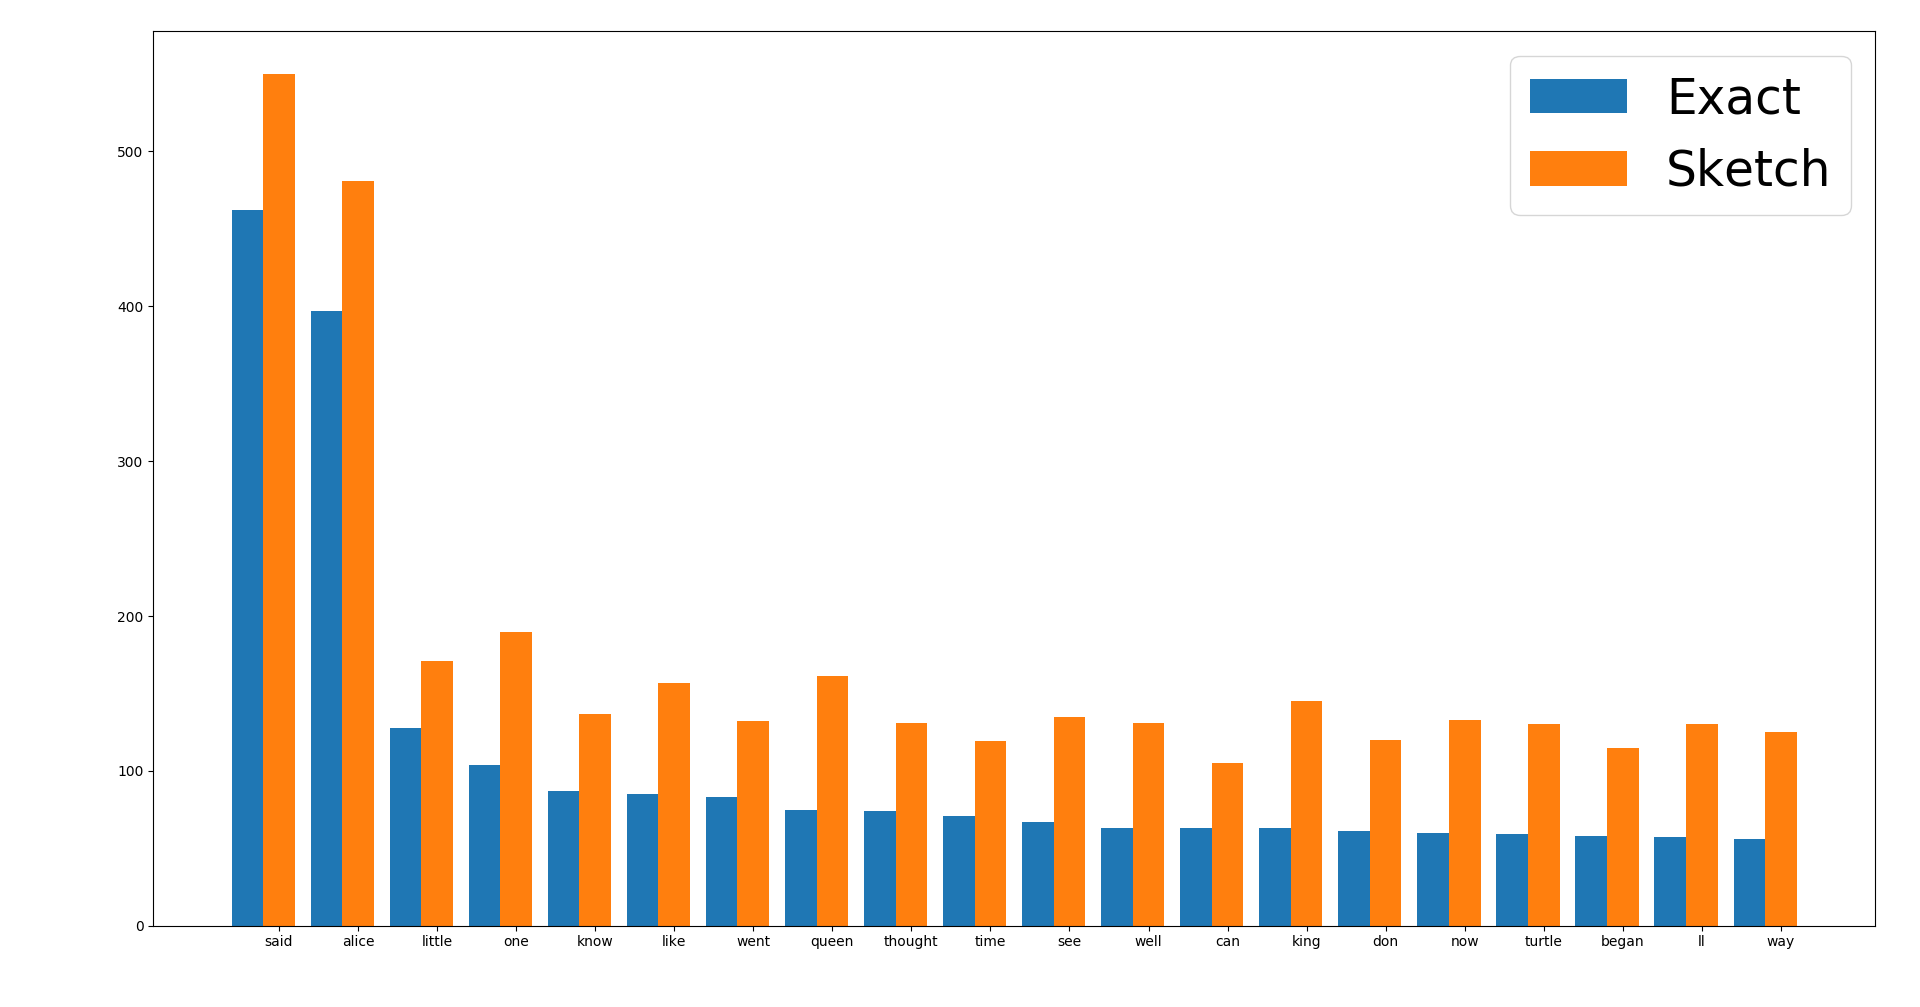
\includegraphics[height=1.6in]{englishAlice100_5.png}
        \caption{Lorem ipsum}
    \end{subfigure}
    \begin{subfigure}[t]{0.5\textwidth}
        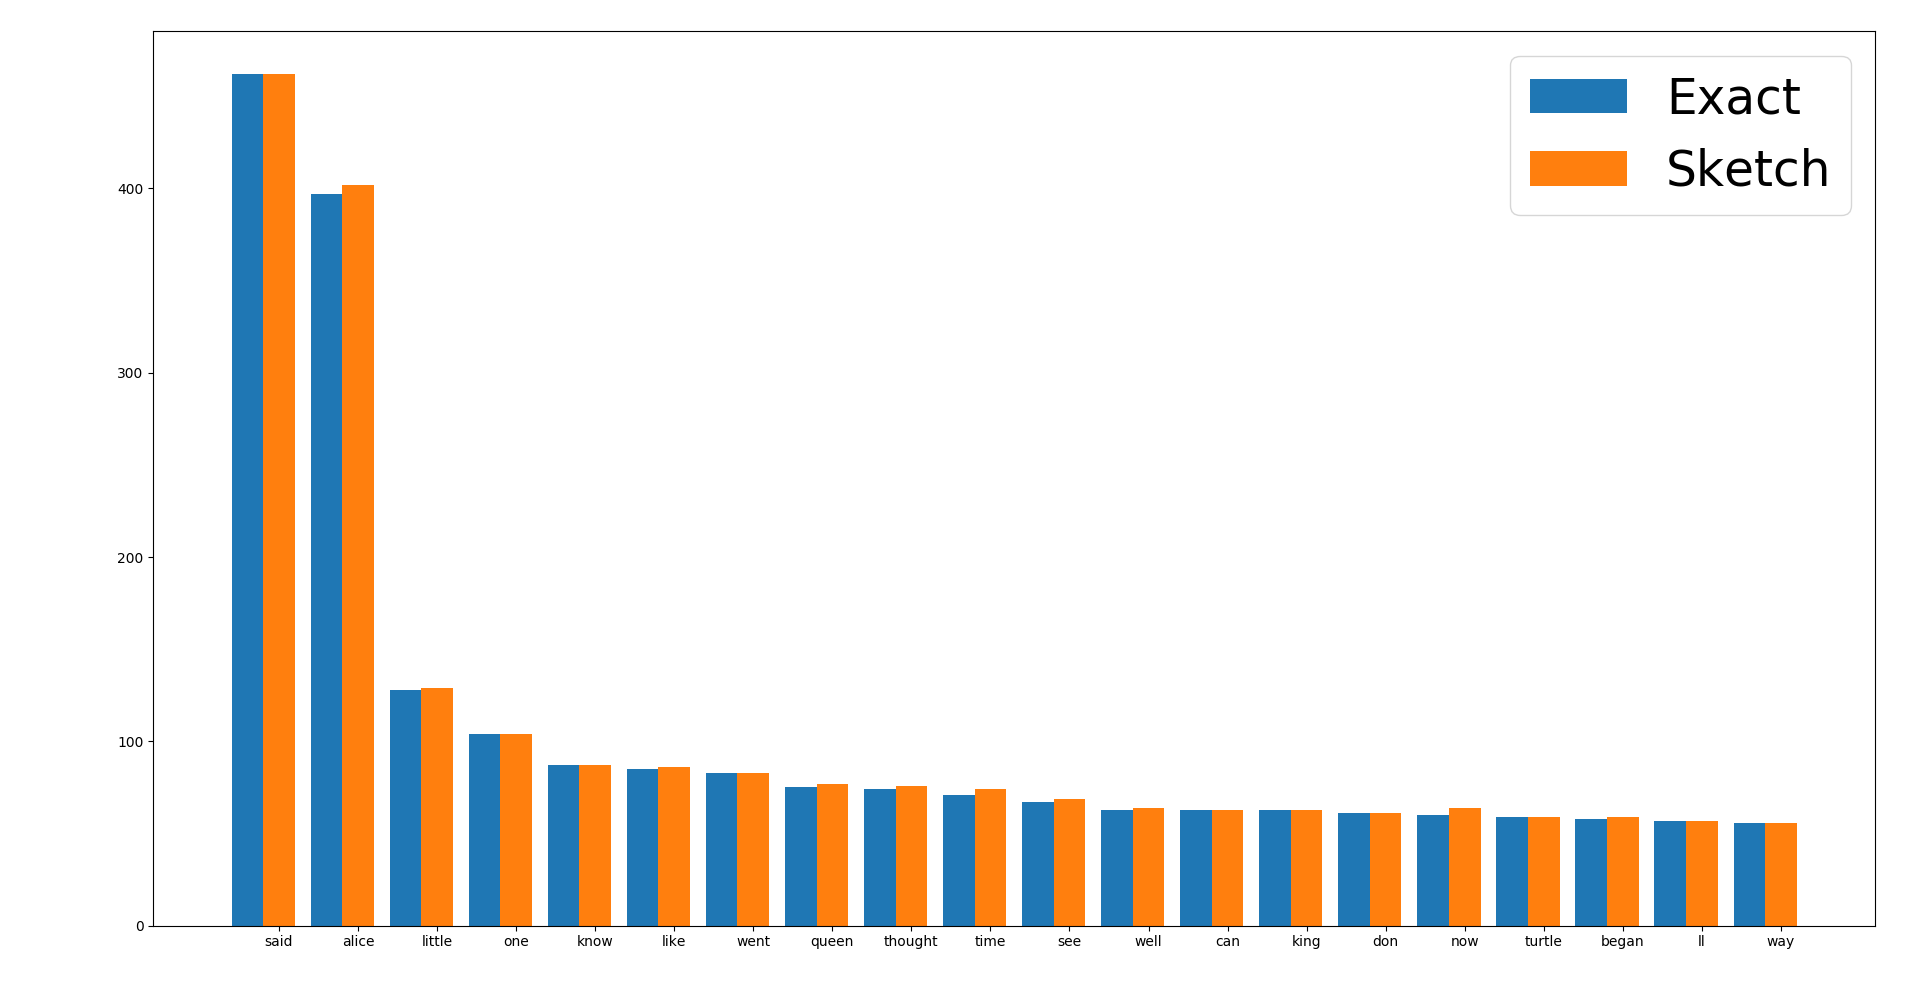
\includegraphics[height=1.6in]{englishAlice1000_5.png}
        \caption{Lorem ipsum}
    \end{subfigure}
    \begin{subfigure}[t]{0.5\textwidth}
        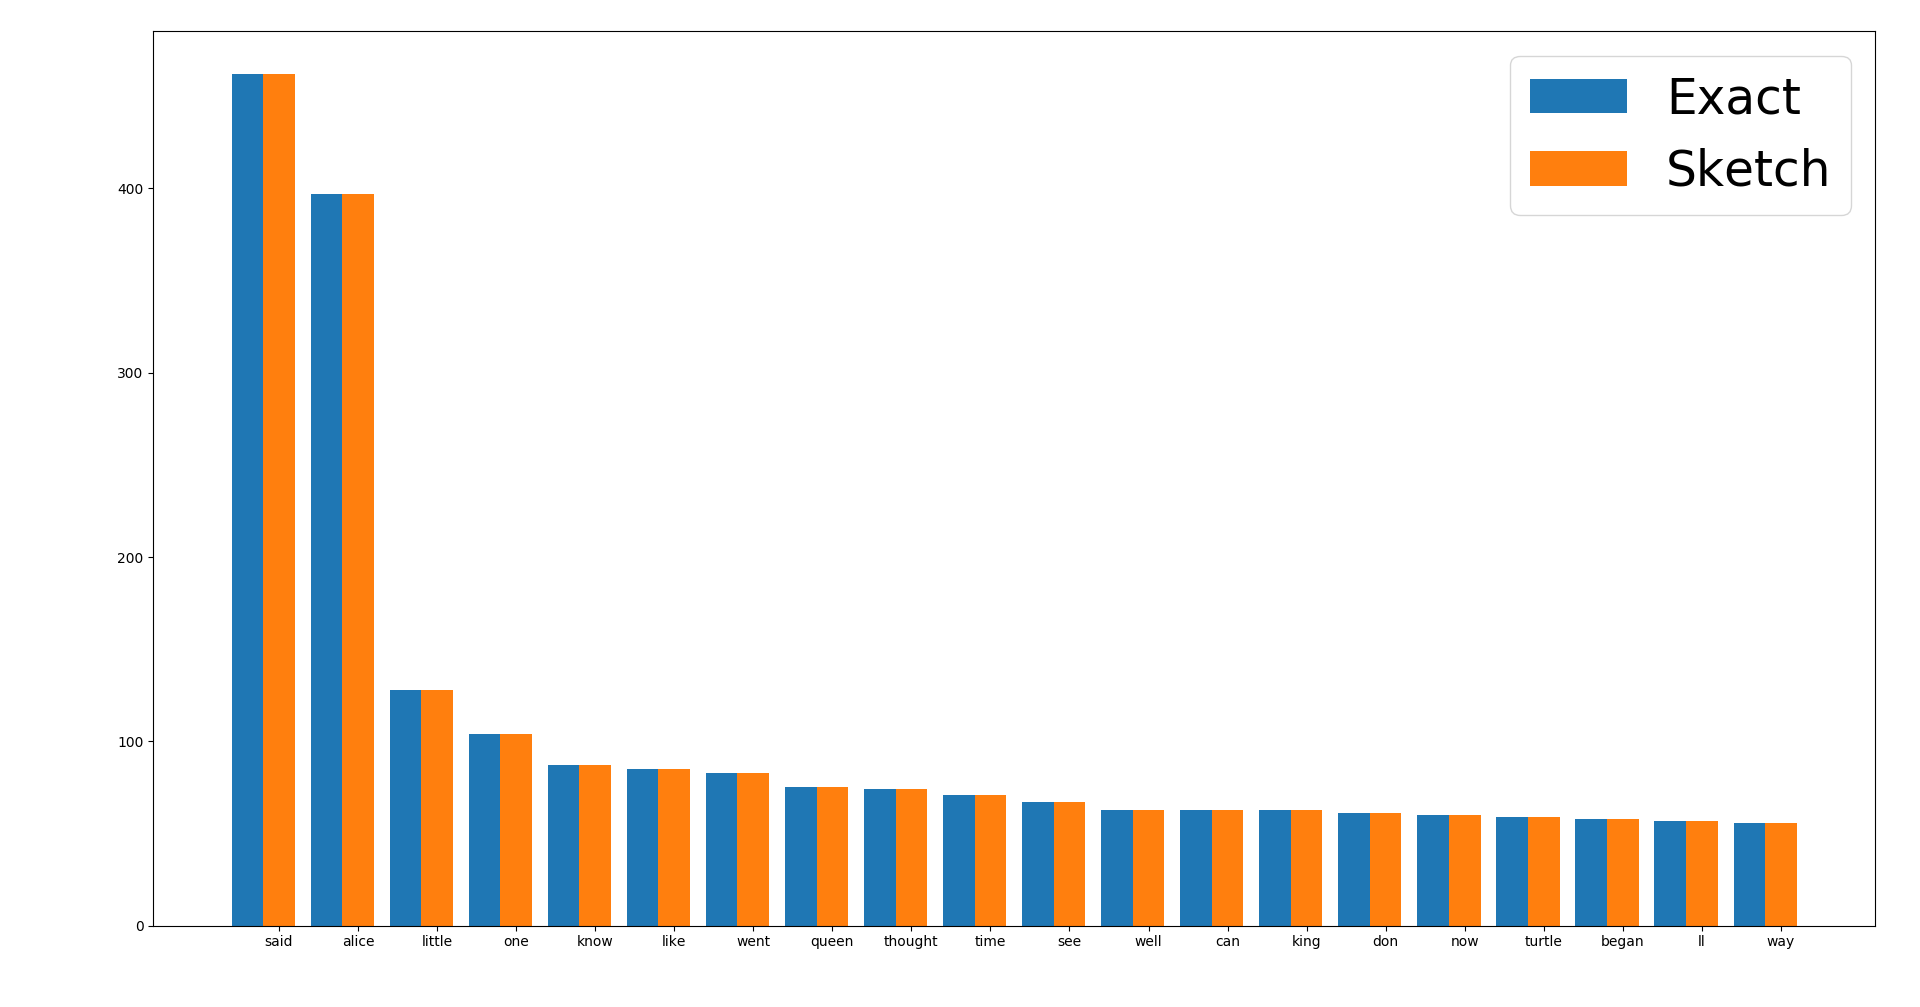
\includegraphics[height=1.6in]{englishAlice10000_5.png}
        \caption{Lorem ipsum}
    \end{subfigure}
    \begin{subfigure}[t]{0.5\textwidth}
        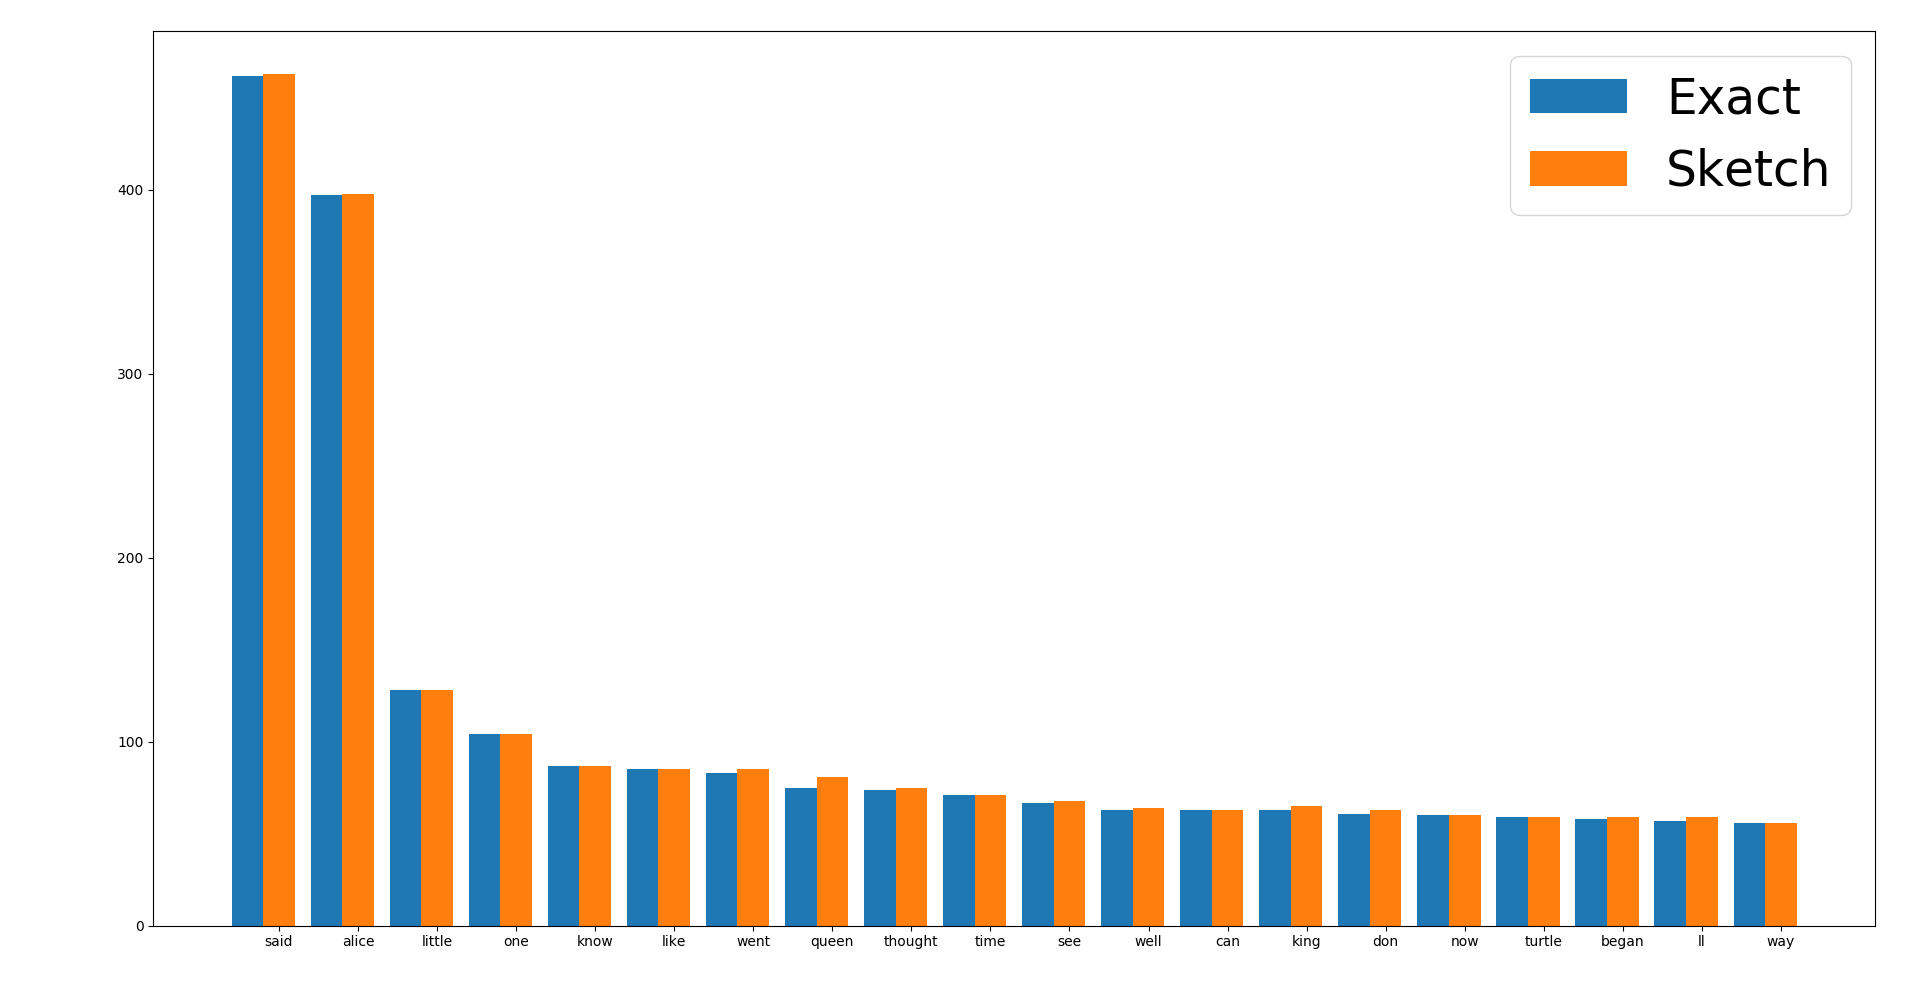
\includegraphics[height=1.6in]{englishAlice1000_6.png}
        \caption{Lorem ipsum}
    \end{subfigure}
    \begin{subfigure}[t]{0.5\textwidth}
        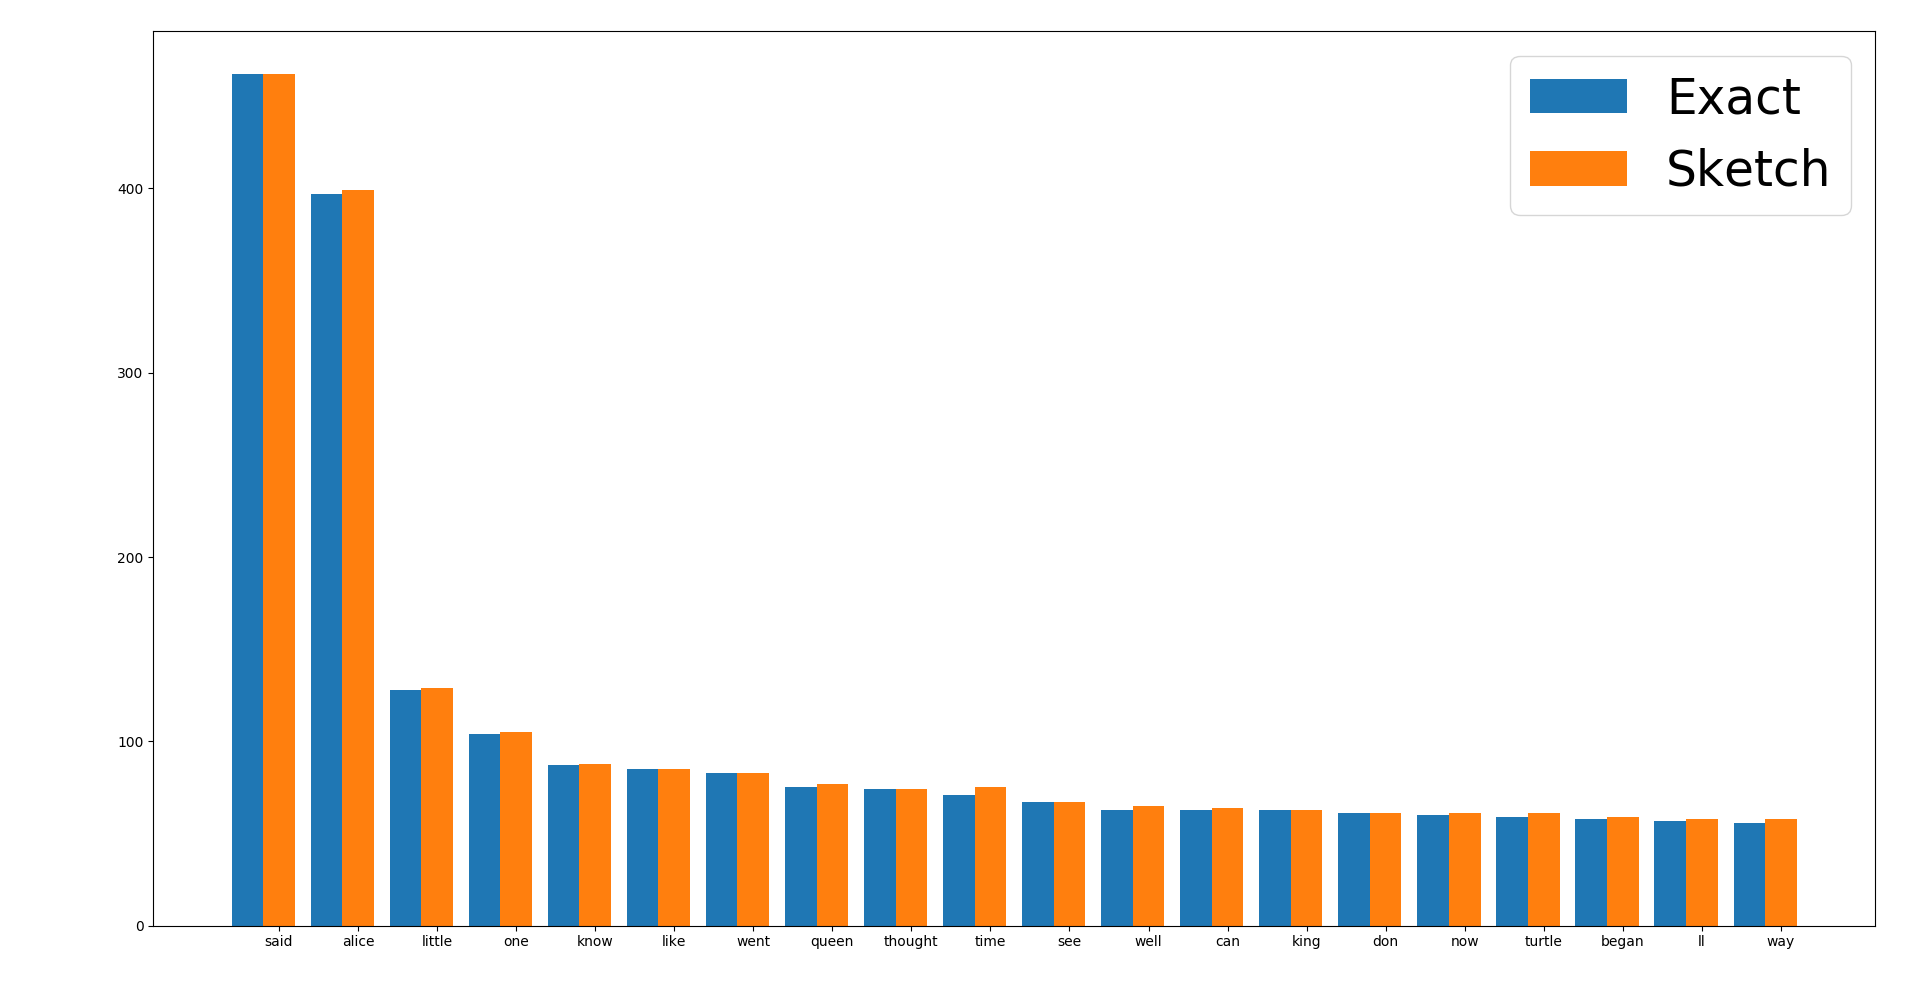
\includegraphics[height=1.6in]{englishAlice1000_8.png}
        \caption{Lorem ipsum}
    \end{subfigure}
    \begin{subfigure}[t]{0.5\textwidth}
        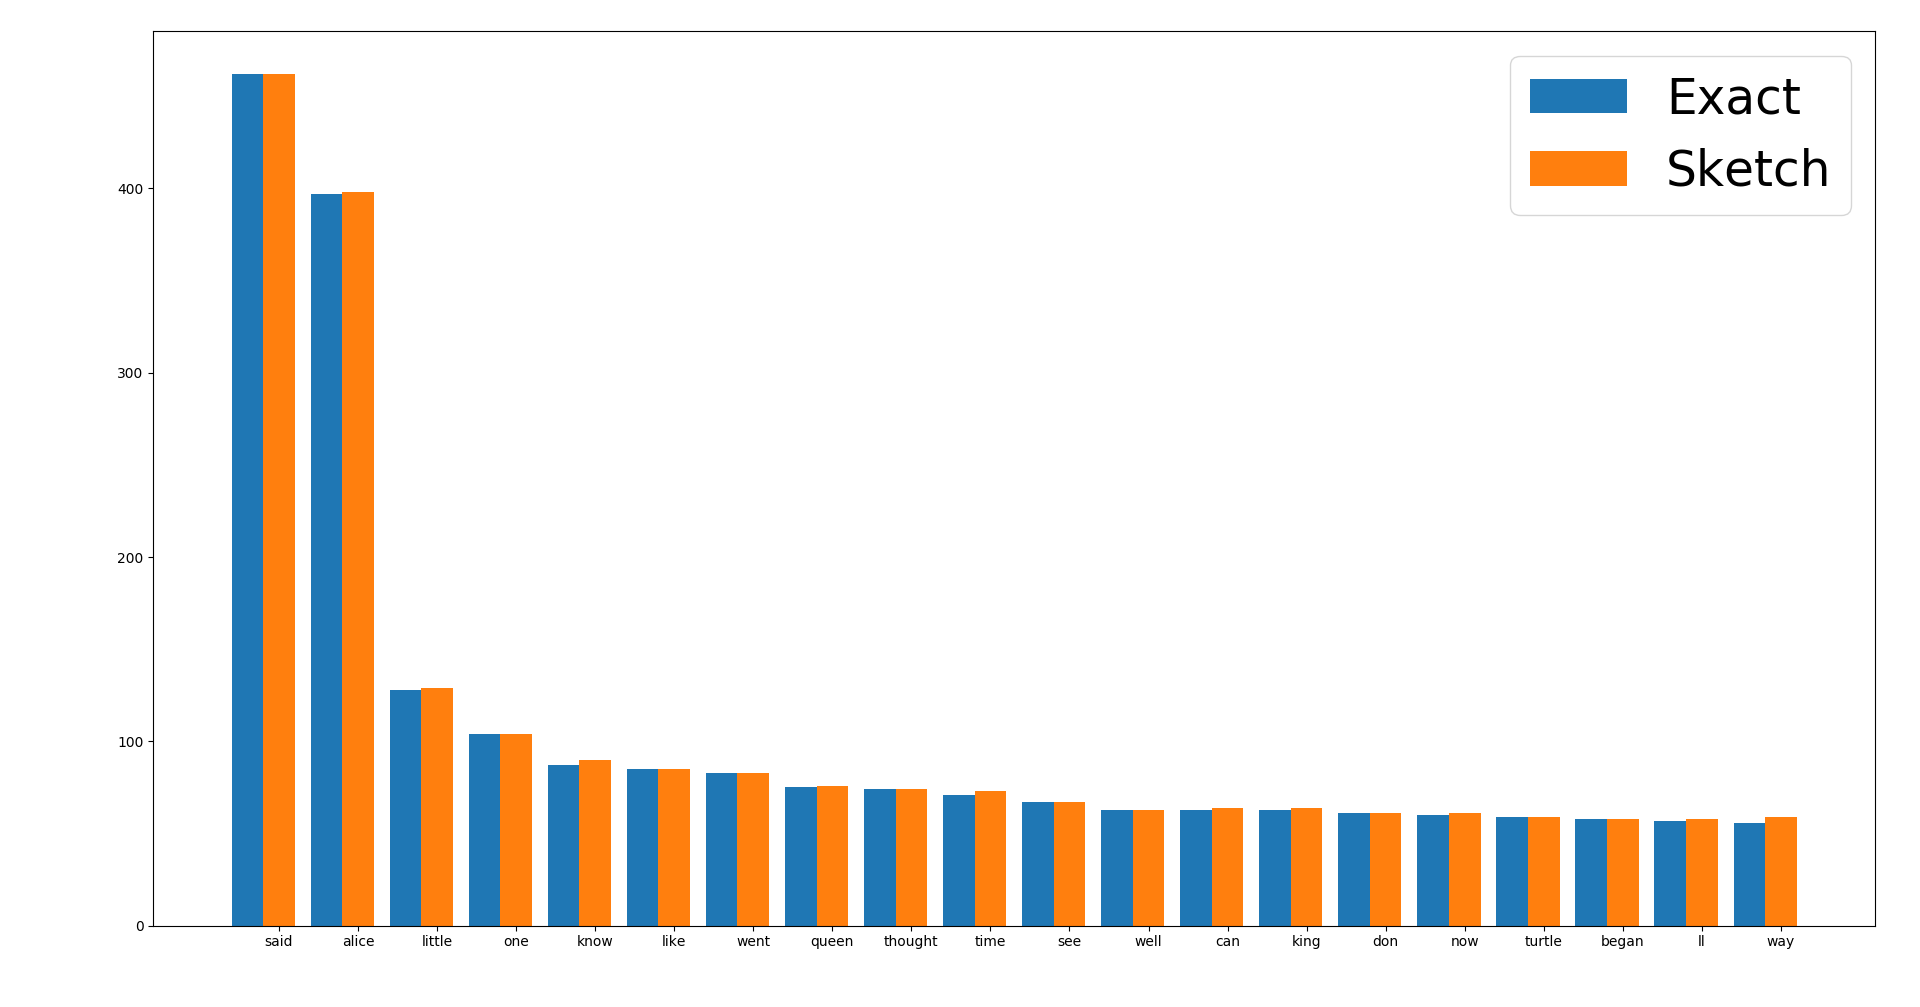
\includegraphics[height=1.6in]{englishAlice1000_10.png}
        \caption{Lorem ipsum}
    \end{subfigure}
    \caption{Caption place holder}
\end{figure*}
%%%%%%%%%%%%%%%%%%%%%%%%%%%%%%%%%%%%%%%%%%%%%%%%%%%%%%%%%%%%%%%%%%%%%%%%%%%%%%%%

\section{Results \& Discussion}

Lorem ipsum ...

% \begin{table}[h!]
% \centering
% \begin{tabular}{@{}c|ccc@{}}
% \toprule
%                       & \textbf{EC} & \textbf{ACFP} & \textbf{ACLP} \\ \midrule
% \textbf{All Words}    & 5116614     & 4886294       & 4797502 \\
% \textbf{Top 10 Words} & 40899       & 22916         & 6635    \\ \bottomrule
% \end{tabular}
% \caption{Number of bytes used in the counter values.}
% \end{table}
% \vspace{-12pt}

% \vspace{-10pt}
% \captionsetup[figure]{labelformat=empty}
% \begin{figure}[H]
%     \centering
%     \setlength{\belowcaptionskip}{-12pt}
%     \includegraphics[width=\linewidth]{wordCount_ACC_DU.png}
%     \caption{Fig. 1: Counter estimations for the top 10 words.} 
%     \label{fig:1}
% \end{figure}

%%%%%%%%%%%%%%%%%%%%%%%%%%%%%%%%%%%%%%%%%%%%%%%%%%%%%%%%%%%%%%%%%%%%%%%%%%%%%%%%

\section{Conclusion}

Lorem ipsum ...

%%%%%%%%%%%%%%%%%%%%%%%%%%%%%%%%%%%%%%%%%%%%%%%%%%%%%%%%%%%%%%%%%%%%%%%%%%%%%%%%

\bibliography{report.bib} 

%\section*{Appendix}

\end{document}
